\documentclass[12pt,english]{article}

% Load citation first, so that footmisc can change footnote, otherwise chicago style footnote overrides footmisc from biblatex-chicago
% https://tex.stackexchange.com/a/110401/109818
%%%%%%%%%%%%%%%%%%%%%%%%
%% SEC: Bibliography %%
%%%%%%%%%%%%%%%%%%%%%%%%
\usepackage[authordate,
backend=bibtex,
doi=false,
isbn=false,
sorting=nyt,
maxbibnames=10,
maxcitenames=3,
sortcites=False]{biblatex-chicago}


% \bibliography{../_bib/ref_one, ../_bib/ref_two, ../_bib/ref_three, ../_bib/ref_four, ../_bib/ref_five}

\AtEveryBibitem{\clearlist{note}\clearlist{language}\clearlist{issn}} % clears issn
\AtEveryBibitem{%
	\ifentrytype{online}{%
		\clearfield{urlyear}
		\clearfield{urlmonth}
		\clearfield{urlday}
		\clearfield{note}
		\clearlist{language}
	}{%
		\clearfield{eprint}%
		\clearfield{url}%
		\clearfield{urlyear}
		\clearfield{urlmonth}
		\clearfield{urlday}
		\clearfield{note}
		\clearlist{language}
	}
}%

% \renewcommand*{\bibfont}{\small}

%%%%%%%%%%%%%%%%%%%%%%%%%
%% SEC: PACKAGEs MAIN  %%
%%%%%%%%%%%%%%%%%%%%%%%%%
\usepackage{mathptmx}
\usepackage{microtype}
\usepackage{amsmath}
\usepackage{bbm}
\usepackage[utf8]{inputenc}
\usepackage[T1]{fontenc}
\usepackage{babel}
\usepackage{setspace}
\usepackage{graphicx}
\usepackage{booktabs,dcolumn}
\usepackage{array}
\usepackage{multirow}
\usepackage[usenames,dvipsnames,svgnames,table]{xcolor}
\usepackage[export]{adjustbox}[2011/08/13]
\usepackage{enumitem}
% FOOTMISC: https://tex.stackexchange.com/a/110401/109818, loading biblatex-chicago after footmisc over-rides footmisc.
\usepackage[hang, flushmargin, bottom, symbol]{footmisc}
\usepackage[text={16cm,24cm}]{geometry}
\usepackage{ragged2e}
\usepackage{csquotes}
\usepackage[colorlinks=true, linkcolor=blue, citecolor=blue, plainpages=false, pdfpagelabels=true, urlcolor=blue]{hyperref}
\usepackage{float}
\usepackage{blindtext}

%%%%%%%%%%%%%%%%%%%%%%%%%%%%%%%%%%
%% For Subfigure alignment and Labeling
%%%%%%%%%%%%%%%%%%%%%%%%%%%%%%%%%%
% \usepackage{subfig}
% \usepackage[font=singlespacing, skip=10pt]{caption}
\usepackage{subcaption}
\usepackage{caption}
\captionsetup[figure]{labelfont={bf},name={Fig.},labelsep=period}
% http://www.peteryu.ca/tutorials/publishing/latex_captions
% Alph for A, B, C, ... 
\renewcommand\thesubfigure{\textbf{\alph{subfigure}}}
% simple format: no parenthesis around (A) (B)
% captionskip: gap between panel sub-eheading and figure
% \captionsetup[subfigure]{labelformat=simple, labelsep=space, captionskip=0pt}


%%%%%%%%%%%%%%%%%%%%%%%%%
%% SEC: Indentation  %%
%%%%%%%%%%%%%%%%%%%%%%%%%
\geometry{
	a4paper,
	noheadfoot=true,
	left=1.0in,
	right=1.0in,
	top=1.0in,
	bottom=1.0in,
}
\makeatletter
%\date{Janunary 2, 2018}
% \date{April 15, 2021}
\date{September 8, 2021}
%\date{}

%%%%%%%%%%%%%%%%%%%%%%%%%
%% SEC: new commands  %%
%%%%%%%%%%%%%%%%%%%%%%%%%
%\exhyphenpenalty=10000\hyphenpenalty=10000
\newcommand\invisiblesection[1]{%
	\refstepcounter{section}%
	\addcontentsline{toc}{section}{\protect\numberline{\thesection}#1}%
	\sectionmark{#1}}

\newcommand{\rowgroup}[1]{\hspace{-0.5em}#1}

\newcolumntype{L}[1]{>{\raggedright\let\newline\\\arraybackslash\hspace{0pt}}m{#1}}
\newcolumntype{C}[1]{>{\centering\let\newline\\\arraybackslash\hspace{0pt}}m{#1}}
\newcolumntype{R}[1]{>{\raggedleft\let\newline\\\arraybackslash\hspace{0pt}}m{#1}}

\newcommand*\samethanks[1][\value{footnote}]{\footnotemark[#1]}
\newcommand{\sym}[1]{\ifmmode^{#1}\else\(^{#1}\)\fi}

%%%%%%%%%%%%%%%%%%%%%%%%
%% SEC: Footer  %%
%%%%%%%%%%%%%%%%%%%%%%%%
\usepackage{calc}
\setlength{\footskip}{\paperheight
	-(1in+\voffset+\topmargin+\headheight+\headsep+\textheight)
	-0.75in}

%%%%%%%%%%%%%%%%%%%%%%%%%%%%%%%%%%%%%%%%%%%%%%%%%
%%% Remove the spacing between paragraphs and have a small paragraph indentation
%%%%%%%%%%%%%%%%%%%%%%%%%%%%%%%%%%%%%%%%%%%%%%%%%
\setlength{\parskip}{0cm}
\setlength{\parindent}{15pt}

%%%%%%%%%%%%%%%%%%%%%%%%%%%%%%%%%%%%%%%%%%%%%%%%%
%%% Line Spacing for Main Text and Footnotes
%%%%%%%%%%%%%%%%%%%%%%%%%%%%%%%%%%%%%%%%%%%%%%%%%

%Using the setspace package:
%\setstretch{1.5}
\doublespacing
%\onehalfspacing

%%%%%%%%%%%%%%%%%%%%%%%%%%%%%%%%%%%%%%%%%%%%%%%%%
%%% Footnotes
%%%%%%%%%%%%%%%%%%%%%%%%%%%%%%%%%%%%%%%%%%%%%%%%%
% 1. Number hang with gap
% 2. Gap between citations
% 3. linespae

\usepackage{footnotebackref}
% separation between foonotes
\addtolength{\footnotesep}{1.5mm}
% within footnote separation
\renewcommand{\footnotelayout}{\setstretch{1.10}}%
\setlength{\footnotemargin}{3.5mm}


%%%%%%%%%%%%%%%%%%%%%%%%%%%%%%%%%%%%%%%%
% 1. Define Keywords, JEL
%%%%%%%%%%%%%%%%%%%%%%%%%%%%%%%%%%%%%%%%
\newcommand{\PAPERKEYWORDS}{\textbf{Keywords}: Early Childhood, Height, Reference Points, Nutrition, Anthropometrics}
\newcommand{\PAPERJEL}{\textbf{JEL}: I15, D8, D9, O15}

%%%%%%%%%%%%%%%%%%%%%%%%%%%%%%%%%%%%%%%%
% 2. Define Title
%%%%%%%%%%%%%%%%%%%%%%%%%%%%%%%%%%%%%%%%
\newcommand{\PAPERTITLE}{\href{https://papers.ssrn.com/sol3/papers.cfm?abstract_id=3167023}{You are What Your Parents Expect: Height and Local Reference Points}}

%%%%%%%%%%%%%%%%%%%%%%%%%%%%%%%%%%%%%%%%
% 3. Define Authors contact information
%%%%%%%%%%%%%%%%%%%%%%%%%%%%%%%%%%%%%%%%
\newcommand{\AUTHORWANG}{Fan Wang: Department of Economics, University of Houston, Houston, Texas, USA (email: fwang26@uh.edu)}

%%%%%%%%%%%%%%%%%%%%%%%%%%%%%%%%%%%%%%%%
% 4. Define Thanks
%%%%%%%%%%%%%%%%%%%%%%%%%%%%%%%%%%%%%%%%
\newcommand{\ACKNOWLEDGMENTS}{
We thank \blindtext}

%%%%%%%%%%%%%%%%%%%%%%%%%%%%%%%%%%%%%%%%
% 5. Define Abstract
%%%%%%%%%%%%%%%%%%%%%%%%%%%%%%%%%%%%%%%%
\newcommand{\PAPERABSTRACT}{
Recent estimates are that about 150 million children under five years of age are stunted, with substantial negative consequences for their schooling, cognitive skills, health, and economic productivity. Therefore, understanding what determines such growth retardation is significant for designing public policies that aim to address this issue. We build a model for nutritional choices and health with reference-dependent preferences. Parents care about the health of their children relative to some reference population. In our empirical model, we use height as the health outcome that parents target. Reference height is an equilibrium object determined by earlier cohorts' parents' nutritional choices in the same village. We explore the exogenous variation in reference height produced by a protein-supplementation experiment in Guatemala to estimate our model’s parameters. We use our model to decompose the impact of the protein intervention on height into price and reference-point effects. We find that the changes in reference points account for 65\% of the height difference between two-year-old children in experimental and control villages in the sixth annual cohort born after the initiation of the intervention.
\PAPERJEL}


\begin{document}


%%%%%%%%%%%%%%%%%%%%%%%%%%%%%%%%%%%%%%%%
% Part I. Title Page, Authors, Abstract, etc. 
%%%%%%%%%%%%%%%%%%%%%%%%%%%%%%%%%%%%%%%%
\title{
% \vspace*{-3em}
\onehalfspacing
\PAPERTITLE
\thanks{\PAPERINFO}}

\author{
\AUTHORWANG{} and \AUTHORTEXFORECON{}\thanks{
\AUTHORWANGINFO;
\AUTHORTEXFORECONINFO.
\ACKNOWLEDGMENTS
}}

\date{
% \vspace*{-0.5em}
March 19, 2022}

\maketitle

% \vspace*{-2em}
\begin{abstract}
% \vspace*{-0.5em}
\singlespacing
\PAPERABSTRACT
\end{abstract}
\vfil
\hfil \small\PAPERKEYWORDS \hfil
\vfil
\thispagestyle{empty}
\clearpage

%%%%%%%%%%%%%%%%%%%%%%%%%%%%%%%%%%%%
% Part II. Manuscript main text
%%%%%%%%%%%%%%%%%%%%%%%%%%%%%%%%%%%%
\pagenumbering{arabic}
\setcounter{page}{1}
\renewcommand*{\thefootnote}{\arabic{footnote}}
% Manuscript main text
%%%%%%%%%%%%%%%%%%%%%%%%%%%%%%%%%%%
% Main Text
%%%%%%%%%%%%%%%%%%%%%%%%%%%%%%%%%%%
\section{Introduction}

Insufficient height and weight growth still affect many children around the globe. Estimates are that about 150 million (22 percent) of children under five years of age are stunted \autocite{fao_state_2019}.\footnote{Stunted children have height-for-age more than two standard deviations below the median for a well-nourished population. In 2018, 59 million (30 percent) and 82 million (23 percent) of African and (non-Japanese) Asian children under five years of age were stunted, respectively \autocite{fao_state_2019}.} Studies suggest that these children are at risk of not developing their full human capital potential \autocite{behrman_nutritional_2009, black_early_2017, hoddinott_effect_2008, hoddinott_adult_2013, hoddinott_economic_2013, maluccio_impact_2009, richter_investing_2017, victora_maternal_2008}. Our paper contributes to a growing literature that investigates how interventions in early childhood can contribute to foster human-capital formation for at-risk children \autocite[e.g.,][]{carneiro_heckman_2003, cunha_heckman_2007, cunha_heckman_jeea, cunha_heckman_schennach_2010, heckman_etal_jpube2010, heckman_etal_qe2010, heckman_etal_aer2010, campbell_etal_2014, gertler_etal_2014}.

\section{The Model}

Following our discussions on parental beliefs, given $\Omega_{y,v} = \big(Y, p^{N}_{yv}, \delta, X, \epsilon, \mu_{R_{y,v}}, \sigma_{R_{y,v}}^{2} \big)$, each household solves the following maximization problem:

\begin{equation}
\label{eq:optimain}
\max_{C,N} \Bigg\{C+\rho\cdot C^{2}+  \left\{ \gamma\cdot H^{24}+\lambda \cdot \int_{R_{yv}} \left(H^{24}-R_{yv}\right)\mathbbm{1}\left\{ H^{24}\ge R_{yv}\right\}\phi \left(R_{yv};\mu_{R_{yv}}, \sigma_{R_{yv}}^{2} \right) dR_{yv} \right\} \Bigg\}
\end{equation}

subject to the budget constraint \eqref{eq:budget_constraint}, the production function \eqref{eq:prod_function}, the equation that determines mean \eqref{eq:mean_belief}, and some measure of variance beliefs $\sigma^2_{R_{y,v}}$. Let $N\left(\Omega_{y,v}\right)$ denote the policy function for nutrition. If $\sigma^2_{R_{y,v}}=0$, preferences for health would be piecewise linear with a kink at $\mu_{R_{yv}}$. If $\sigma^2_{R_{y,v}}>0$, preferences for health are continuously differentiable; if additionally $\gamma>0$ and $\lambda<0$, preferences for health are concave.

The optimization problem in Equation \eqref{eq:optimain} does not permit analytical solutions.\footnote{In Appendix Section \ref{sec:apprefsd}, we discuss the first-order condition for the optimal nutritional choice problem. In Appendix Section \ref{sec:modelsolu}, we describe the procedures for numerical solutions.} To illustrate how changes in key parameters impact optimal choices, we present in Figure \ref{fig:indiff} the consumption-health possibility frontier along with several indifference curves for an individual, using estimated parameters from our model.\footnote{The consumption-health possibility frontier is jointly determined by the household budget and the child height production function.} In each panel, solid dots indicate optimal choices (i.e., the combination of height and household consumption where indifference curves are tangent to the consumption-health possibility frontier).

Panel a shows several indifference curves and the consumption-health possibility frontier. The figure clearly shows the asymmetry in indifference curves. To the left of the mean reference height, parents are willing to sacrifice a large amount of consumption for a small increase in the child's height. In contrast, to the right of the mean reference height, parents are willing to forego only a small amount of consumption for a large increment in height.

In panel b, we vary the $\lambda$ parameter. Marginal benefits of additional nutritional intakes on expected utility are increasing in $\lambda$. Additionally, reference points matter more when $\lambda$ deviates more from zero. Visually, at more negative values of $\lambda$, the curvature of the indifference curve increases. The greater the curvature of the indifference curve, the more critical the role of reference height in determining parental nutritional choices and, consequently, the child's height at age 24 months.

In panel b, we fix $\lambda$ and vary $\mu_{R_{y,v}}$. When $\lambda<0$, the marginal benefits of additional nutritional intakes are increasing in $\mu_{R_{y,v}}$. The greater the value of $\mu_{R_{y,v}}$, the lower the household consumption and the taller the child at age 24 months.

Finally, panel d of Figure \ref{fig:indiff} presents the effect of increasing uncertainty about the parental estimates of mean height, $\sigma^2_{R_{y,v}}$. Given the estimated parameters from the empirical model, higher values of $\sigma^2_{R_{y,v}}$ increase the marginal benefits of additional nutrition when expected height exceeds $\mu_{R_{y,v}}$ and reduces the curvature of the indifference curves. These lead to an increase in nutritional choices. In the limit, as $\sigma^2_{R_{y,v}}$ approaches infinity, preferences become linear in height, and predictions from models with and without reference points become empirically indistinguishable.

We use the estimated parameters to produce Figure \ref{fig:indiff}. However, in general, the household response to an increase in uncertainty depends on the values of $\gamma$ and $\lambda$. When marginal utility gains from additional investment in health are positive after the mean reference point $\mu_{R}$ -- which means $-\gamma < \lambda < 0$ -- an increase in $\sigma_{R}$ will lead to an increase in investments in health. In contrast, if marginal utility from additional investment in health is negative after the mean reference point $\mu_{R}$ -- which generates backward bending indifference curves -- a similar increase of $\sigma_{R}$ could reduce investment in health. Ceteris paribus, there is a threshold level of $\lambda$ where increases in $\sigma_{R}$ have no impact on health investments. In Appendix Section \ref{sec:apprefsd}, we discuss the intuition behind these results and provide graphical illustrations.


\section{Data}


The data we use in this paper comes from an experimental intervention conducted by The Institute of Nutrition of Central America and Panama (INCAP), which started a nutritional-supplementation trial in 1969. Four villages from eastern Guatemala were selected, one pair of villages that was relatively populous (\textasciitilde900 residents each) and one pair that was less populous (\textasciitilde500 residents each). The villages were similar in child nutritional status, measured as the height at three years of age \autocite{habicht_nutritional_1995}. Over 50\% of children lacked proper nutrition and were severely stunted, measured as height-for-age z-scores less than -3.\footnote{Guatemalan children continue to suffer from severe malnutrition. In 2015, among Guatemalan households in the lowest quintile of wealth, approximately 70 percent of children younger than five were stunted. In middle-quintile Guatemalan households, 45 percent of children younger than five were stunted \autocite{fao_state_2019}.} The intervention consisted of randomly assigning nutritional supplements. One large and one small village were selected to receive a high-protein drink called Atole, and the other two were selected to receive an alternative supplement called Fresco. Each serving of Atole (180 ml) contained 11.5 grams of protein and 163 kcal. Fresco had no proteins, and each serving (180 ml) had 59 kcal. The central hypothesis was that the protein supplementation would accelerate physical and mental development \autocite{habicht_nutritional_1995}. The intervention started in February 1969 in the larger villages and in May 1969 in the smaller villages and lasted until the end of February 1977, with data collection taking place until September 1977 \autocite{maluccio_impact_2009,islam_evidence_2009}. The nutritional supplements were distributed in feeding centers located centrally in each village. The centers were open twice a day, two to three hours in the mid-morning and two to three hours in the mid-afternoon. All village members had access to the supplements at the feeding centers.

Table \ref{summcovarmain} presents summary statistics for the variables that we use in our analysis. In Panels a and b, we show statistics on gender, income, and prices for our main sample of 503 individuals (panel a) and gender and income for the fuller sample of 1155 individuals (panel b). In Panels c and d, we show statistics on heights and nutritional intakes, respectively. Table \ref{summcovarmain} has five columns. The first column presents the overall means and standard deviations in Atole and Fresco villages combined. The second and third columns present Atole and Fresco village-specific means and standard deviations. Column four shows the gaps in means between Atole and Fresco villages for each variable, and column five presents the p-values for the statistical significance of these gaps.

As mentioned before, the intervention took place in four villages, two Atole or treatment villages and two Fresco or control villages. In the rest of the paper, when we refer to Atole and Fresco villages, we merge the information of the two villages that received the same supplement. The limited number of villages might impact the descriptive statistics' standard errors since villages can share common unobserved shocks. We follow the methods developed by \textcite{donald2007inference} and \textcite{cameron2015practitioner} to study how robust our results are to this clustering. The method proposed by \textcite{donald2007inference} consists of estimating averages by clusters, controlling for individual variables, and using those averages in the regressions. This method greatly reduces the number of observations. We define cluster year-village pairs and half-year-village pairs to implement this procedure. Following \textcite{cameron2015practitioner} we also implement a pair-cluster bootstrap, using the same cluster definition as in the \textcite{donald2007inference} method. Table \ref{summcovarmain} and Figure \ref{fig:PortHgtGap} report the results without using the clusters corrections, but the results are robust to those methods.

\section{Results}


We present estimated parameters in Table \ref{tab:paramestitwo}, with standard errors shown in parentheses. For preferences, $\rho$ is -0.047, indicating that preferences are concave in $c$. $\gamma$ and $\lambda$ are $0.033$ and $-0.026$, respectively. Therefore, preferences are also concave in height, and the curvature of the indifference curves indicates the asymmetry in responses. Parents prefer taller to shorter children, but the marginal benefit from an additional centimeter of height beyond the reference comparison height is close to zero (albeit positive).

The price discount parameter $\delta$ is $0.376$, representing a $38\%$ discount in protein prices in Atole villages. The production-function parameters are $\beta=0.073$, $\alpha_{H_0}=0.022$, $\alpha_{male}=0.009$, $A=4.144$, and $\sigma_{\epsilon}=0.010$. Given these parameters, we show the consumption- and height-possibility frontier along with indifference curves for an individual in panel a of Figure \ref{fig:indiff}.

The measurement-error estimates are $\sigma_{\eta}=0.382$ and $\sigma_{\iota}=0.043$. These findings indicate that measurement error is more severe for nutritional intake than height, which is intuitive.

We use the estimated model to decompose the relative contributions of prices and reference points to the height dynamics in Atole and Fresco villages. In Appendix \ref{sec:targetuniversal}, we discuss additional counterfactuals in which we compare the relative impacts of poor-targeted and universal policy experiments given reference points.


\section{Conclusion}

In this paper, we build and estimate a child-nutritional investment model. The model considers reference-dependent preferences, where the reference is with respect to the heights of the previous cohort of children who live in the same village. Reference points shift endogenously as households observe children’s heights from earlier birth cohorts changing.

For researchers interested in the impact of price subsidies and income transfers, we have introduced a long-term secondary channel -- endogenous changes in reference points -- that might affect the impacts of these policies. For the protein-supplement experiment implemented in Guatemala, which we interpret as a price-discount policy, by 1975 -- six years after the start of the policy – 57\% to 65\% of the policy’s impact are due to its impact on shifting reference points.

Our paper also shows significant height increases might be realized from shifting reference points for highly-stunted populations. It is an open question how to exogenously shift these reference points in the short run, although the Peruvian experience mentioned in the introduction indicates that educational campaigns could be effective on a large scale over time. The cost of an educational campaign to inform households about alternative reference heights well might be lower compared to income transfers and price subsidies with similar effects on heights.

We recognize that our analysis requires a crucial assumption: parents use the data on a selected group of children to estimate mean and variance beliefs about the reference height. We argued that our assumption is consistent with research in economics, medicine, and anthropology, but we recognize that there are many other alternatives, such as rational expectations, Bayesian updating, or social learning models. Unfortunately, the literature in economics knows very little about such a critical element of the model we propose in this paper. Therefore, it is necessary to encourage research that elicits parental subjective distributions of reference points as part of parent-directed interventions to reduce stunting. Within a randomized controlled trial, the availability of such data would shed light on the process parents use to update critical moments of the subjective distribution. With such evidence, one could have a more robust representation of our model that would better inform the design of public policies to improve children’s health.
\clearpage

%%%%%%%%%%%%%%%%%%%%%%%%%%%%%%%%%%%
% Part III. Bibliography
%%%%%%%%%%%%%%%%%%%%%%%%%%%%%%%%%%%
\begingroup
\setstretch{1}
\setlength\bibitemsep{5pt}
\printbibliography[title=References]
\endgroup
\pagebreak

%%%%%%%%%%%%%%%%%%%%%%%%%%%%%%%%%%%%
% Part IV. Tables and figures
%%%%%%%%%%%%%%%%%%%%%%%%%%%%%%%%%%%%
%%%%%%%%%%%%%%%%%%%%%%%%%%%%%%%%%%%%
% Figures
%%%%%%%%%%%%%%%%%%%%%%%%%%%%%%%%%%%%

% Figure 1
\newcommand{\subFigWidth}{0.50}
\begin{figure}[H]
    \centering
    \begin{subfigure}[b]{\subFigWidth\textwidth}
        \centering
        \includegraphics[width=\linewidth]{\string"fig_main/fig1a_Tester_Indiff_person_495_med_2021".eps}
        \caption{Contours of indifference curves at given estimates}
    \end{subfigure}~
	\begin{subfigure}[b]{\subFigWidth\textwidth}
	    \centering
    	\includegraphics[width=\linewidth]{\string"fig_main/fig1b_Tester_Indiff_person_495_lambdam3_20210130".eps}
    	\caption{Vary $\lambda$}
	\end{subfigure}
	\par\medskip
	\begin{subfigure}[b]{\subFigWidth\textwidth}
        \centering
        \includegraphics[width=\linewidth]{\string"fig_main/fig1c_Tester_Indiff_person_495_refmeanm3_20210130".eps}
        \caption{Vary $\mu_{R}$}
    \end{subfigure}~
	\begin{subfigure}[b]{\subFigWidth\textwidth}
	    \centering
	    \includegraphics[width=\linewidth]{\string"fig_main/fig1d_Tester_Indiff_person_495_refsd_increasem3_20210130".eps}
	    \caption{Vary $\sigma_{R}$}
	\end{subfigure}
	\caption{Consumption and height outcome indifference curves and choice frontiers. \emph{Note}: Health possibility frontier and indifference curves are visualized in blue (solid-line) given estimated parameters and characteristics for one particular child. The consumption and expected height outcome frontier is determined by the budget constraint as well as the production function. Panels b, c and d show results from varying one parameter at a time in red (dashed-line) and orange (dotted-line). See Section \ref{sec:maximize} for discussions.}
	\label{fig:indiff}
\end{figure}
\pagebreak

% Figure 2
\begin{figure}[H]
    \centering
    \begin{subfigure}[t]{.43\textwidth}
        \centering
        \includegraphics[width=\linewidth]{\string"fig_main/fig2a_ss_mean_hgt24_yr_trimmed".eps}
        \caption{Height}
    \end{subfigure}~
	\begin{subfigure}[t]{0.57\textwidth}
	    \centering
    	\includegraphics[width=\linewidth]{\string"fig_main/fig2b_ss_mean_prot_15t24_yr".eps}
    	\caption{Protein}
	\end{subfigure}
	\caption{Increasing protein and height gaps across cohorts. \emph{Note}: See Section \ref{sec:gap} for discussions.}
	\label{fig:PortHgtGap}
\end{figure}
\pagebreak

\clearpage

%%%%%%%%%%%%%%%%%%%%%%%%%%%%%%%%%%%%
% Tables
%%%%%%%%%%%%%%%%%%%%%%%%%%%%%%%%%%%%
% Table 1
\begin{table}[t!]
{\small
\centering                                 \def\sym#1{\ifmmode^{#1}\else\(^{#1}\)\fi}                                 \caption{Summary statistics for various variables\label{summcovarmain}}                                 \begin{adjustbox}{max width=1\textwidth}                                 \begin{tabular}{m{6.9cm} >{\centering\arraybackslash}m{1.8cm} >{\centering\arraybackslash}m{1.8cm} >{\centering\arraybackslash}m{1.8cm} >{\centering\arraybackslash}m{1.8cm} >{\centering\arraybackslash}m{1.8cm}}                                 \toprule                                                                                         & \multicolumn{5}{C{9cm}}{Atole and Fresco villages differences} \\                                                 \cmidrule(l{5pt}r{5pt}){2-6}                                                   & \multicolumn{1}{C{1.8cm}}{\small \textbf{All}} & \multicolumn{2}{C{3.6cm}}{\small \textbf{Group averages}} & \multicolumn{2}{C{3.6cm}}{\small \textbf{p-values testing}} \\                                                  \cmidrule(l{5pt}r{5pt}){2-2} \cmidrule(l{5pt}r{5pt}){3-4} \cmidrule(l{5pt}r{5pt}){5-6}                                                  & \multicolumn{1}{C{1.8cm}}{\textit{\small mean (sd)}} & \multicolumn{1}{C{1.8cm}}{\textit{\small Fresco}} & \multicolumn{1}{C{1.8cm}}{\textit{\small Atole}} & \multicolumn{1}{C{1.8cm}}{\textit{\small gap}} & \multicolumn{1}{C{1.8cm}}{\textit{\small p-value}} \\
\midrule
\multicolumn{6}{l}{\vspace*{-3mm}\hspace*{-0mm}\textbf{\normalsize Panel a: Gender income price (N=503, main sample)}} \\                                          &            &            &            &            &            \\
Male                &        0.52&        0.52&        0.52&       -0.00&        0.92\\
                    &\vspace*{-2mm}{\footnotesize (0.50) }&\vspace*{-2mm}{\footnotesize (0.50) }&\vspace*{-2mm}{\footnotesize (0.50) }&            &            \\
Income (quetzale)       &      515.57&      503.68&      526.00&       22.32&        0.59\\
                    &\vspace*{-2mm}{\footnotesize (460.9) }&\vspace*{-2mm}{\footnotesize (464.4) }&\vspace*{-2mm}{\footnotesize (458.4) }&            &            \\
Mth 15-24 protein price (quetzale/10k grams)&       52.58&       52.47&       52.68&        0.21&        0.54\\
                    &\vspace*{-2mm}{\footnotesize (3.87) }&\vspace*{-2mm}{\footnotesize (3.93) }&\vspace*{-2mm}{\footnotesize (3.81) }&            &            \\
\midrule
\multicolumn{6}{l}{\vspace*{-3mm}\hspace*{-0mm}\textbf{\normalsize Panel b: Gender income (N=1115, height observed once in first 24 months)}} \\                                          &            &            &            &            &            \\
Male                &        0.53&        0.53&        0.53&        0.00&        0.98\\
                    &\vspace*{-2mm}{\footnotesize (0.50) }&\vspace*{-2mm}{\footnotesize (0.50) }&\vspace*{-2mm}{\footnotesize (0.50) }&            &            \\
Income (quetzale)       &      449.49&      444.63&      454.06&        9.43&        0.72\\
                    &\vspace*{-2mm}{\footnotesize (432.3) }&\vspace*{-2mm}{\footnotesize (446.4) }&\vspace*{-2mm}{\footnotesize (419.0) }&            &            \\
\midrule
\multicolumn{6}{l}{\vspace*{-3mm}\hspace*{-0mm}\textbf{\normalsize Panel c: Height}} \\                                          &            &            &            &            &            \\
Month 0 (cm)  {\footnotesize N=503}&       49.64&       49.79&       49.52&       -0.27&        0.19\\
                    &\vspace*{-2mm}{\footnotesize (2.29) }&\vspace*{-2mm}{\footnotesize (2.29) }&\vspace*{-2mm}{\footnotesize (2.29) }&            &            \\
Month 6 (cm)  {\footnotesize N=463}&       62.72&       62.49&       62.93&        0.44&        0.05\\
                    &\vspace*{-2mm}{\footnotesize (2.46) }&\vspace*{-2mm}{\footnotesize (2.50) }&\vspace*{-2mm}{\footnotesize (2.42) }&            &            \\
Month 12 (cm) {\footnotesize N=475}&       68.81&       68.45&       69.13&        0.68&        0.01\\
                    &\vspace*{-2mm}{\footnotesize (2.99) }&\vspace*{-2mm}{\footnotesize (3.13) }&\vspace*{-2mm}{\footnotesize (2.83) }&            &            \\
Month 18 (cm) {\footnotesize N=482}&       73.37&       72.88&       73.80&        0.92&        0.00\\
                    &\vspace*{-2mm}{\footnotesize (3.23) }&\vspace*{-2mm}{\footnotesize (3.26) }&\vspace*{-2mm}{\footnotesize (3.15) }&            &            \\
Month 24 (cm) {\footnotesize N=503}&       77.66&       76.97&       78.30&        1.33&        0.00\\
                    &\vspace*{-2mm}{\footnotesize (3.47) }&\vspace*{-2mm}{\footnotesize (3.49) }&\vspace*{-2mm}{\footnotesize (3.33) }&            &            \\
\midrule
\multicolumn{6}{l}{\vspace*{-3mm}\hspace*{-0mm}\textbf{\normalsize Panel d: Average daily nutritional intake}} \\                                          &            &            &            &            &            \\
Month 15 (grams/day) {\footnotesize N=464}&       17.43&       14.29&       20.07&        5.78&        0.00\\
                    &\vspace*{-2mm}{\footnotesize (10.5) }&\vspace*{-2mm}{\footnotesize (9.14) }&\vspace*{-2mm}{\footnotesize (10.9) }&            &            \\
Month 18 (grams/day) {\footnotesize N=461}&       21.52&       18.27&       24.41&        6.14&        0.00\\
                    &\vspace*{-2mm}{\footnotesize (11.4) }&\vspace*{-2mm}{\footnotesize (9.61) }&\vspace*{-2mm}{\footnotesize (12.0) }&            &            \\
Month 21 (grams/day) {\footnotesize N=475}&       24.45&       20.17&       27.99&        7.82&        0.00\\
                    &\vspace*{-2mm}{\footnotesize (11.4) }&\vspace*{-2mm}{\footnotesize (9.03) }&\vspace*{-2mm}{\footnotesize (11.9) }&            &            \\
Month 24 (grams/day) {\footnotesize N=462}&       26.99&       22.51&       31.07&        8.56&        0.00\\
                    &\vspace*{-2mm}{\footnotesize (12.0) }&\vspace*{-2mm}{\footnotesize (9.02) }&\vspace*{-2mm}{\footnotesize (13.0) }&            &            \\
Avg mth 15-24 (grams/day) {\footnotesize N=503}&       22.54&       18.78&       25.84&        7.06&        0.00\\
                    &\vspace*{-2mm}{\footnotesize (8.98) }&\vspace*{-2mm}{\footnotesize (6.43) }&\vspace*{-2mm}{\footnotesize (9.62) }&            &            \\
Avg mth 15-24 (kcal/day)   {\footnotesize N=503}&      691.78&      681.78&      700.55&       18.77&        0.38\\
                    &\vspace*{-2mm}{\footnotesize (236.5) }&\vspace*{-2mm}{\footnotesize (236.2) }&\vspace*{-2mm}{\footnotesize (236.9) }&            &            \\
\bottomrule
\addlinespace[0.5em]
\multicolumn{6}{p{1\textwidth}}{\parbox[t]{1.0\textwidth}{\footnotesize{\emph{Note}: See Section \ref{sec:stat} for discussions.}}}\\
\addlinespace
\end{tabular}
\end{adjustbox}
}
\end{table}

\clearpage
% Table 2
\begin{table}[!ht]
\centering{}
{\small
	\caption{\label{tab:paramestitwo}Estimated model parameters ($\sigma_R =0.50$ cm)}
	\begin{tabular}{crlcrl}
		\toprule
		\multicolumn{6}{c}{\textbf{Parameter estimates (s.e.) }} \\
		\midrule
		\multicolumn{6}{c}{\vspace{-3mm}} \\
		\multicolumn{3}{l}{\textit{Preference}}	& \multicolumn{3}{l}{\textit{Production function}} \\
		\multicolumn{6}{c}{\vspace{-3mm}} \\
		$\rho$  & $-0.0473$  & $(0.0031) $ 	 	&        $A$ & $4.1435$ & $(0.0854)$ \\
		$\gamma$ & $0.0325$  & $(0.0059) $ 	    &    	 $\alpha_{H_0}$ & $0.0220$ & $(0.0088)$ \\
		$\lambda$ & $-0.0257$ & $(0.0056) $      &        $\alpha_{male}$ & $0.0086$ & $(0.0016)$ \\
   		\multicolumn{2}{c}{} 	              & &        $\beta$ & $0.0725$ & $(0.0158)$  \\
   		\multicolumn{2}{c}{} 	              & &        $\sigma_\epsilon$ & $0.0097$ &   $(0.0010)$ \\
		\multicolumn{6}{c}{} \\
		\multicolumn{3}{l}{\textit{Price discount}} & \multicolumn{3}{l}{\textit{Measurement error}} \\
		\multicolumn{6}{c}{\vspace{-3mm}} \\
		$\delta$ & $0.3756$ & $(0.0249)$ & $\sigma_\eta$ & $0.3823$ & $(0.0151)$ \\
   		\multicolumn{2}{c}{} 	              & &        $\sigma_\iota$ & $0.0427$ &   $(0.0017)$ \\
		\multicolumn{6}{c}{\vspace{-3mm}} \\
        \bottomrule
        \addlinespace[0.5em]
        \multicolumn{6}{l}{\footnotesize{\emph{Note}: See Section \ref{sec:data} for discussions.}}\\
	\end{tabular}
}
\end{table}
\clearpage
% Table 3
\newcommand{\sefm}[1]{\vspace*{-2mm}{\footnotesize (#1)}}
\begin{table}[htbp]
\centering
{\small
\def\sym#1{\ifmmode^{#1}\else\(^{#1}\)\fi}
\caption{The fit of the estimated model's simulated choices to data\label{modelfit}}
\begin{adjustbox}{max width=1\textwidth}
\begin{tabular}{m{1.3cm}
>{\centering\arraybackslash}m{0.9cm} 
>{\centering\arraybackslash}m{0.9cm} 
>{\centering\arraybackslash}m{0.9cm} 
>{\centering\arraybackslash}m{0.9cm}
>{\centering\arraybackslash}m{0.9cm}
>{\centering\arraybackslash}m{0.9cm}
>{\centering\arraybackslash}m{0.9cm}
>{\centering\arraybackslash}m{0.9cm}
>{\centering\arraybackslash}m{0.9cm}
>{\centering\arraybackslash}m{0.9cm}
>{\centering\arraybackslash}m{0.9cm}
>{\centering\arraybackslash}m{0.9cm}}
\toprule
& \multicolumn{6}{C{5.4cm}}{\hspace*{-10mm}\textbf{Average protein choices (s.e)}} 
& \multicolumn{6}{C{5.4cm}}{\hspace*{-15mm}\textbf{Average height outcome (s.e)}} \\
\cmidrule(l{5pt}r{5pt}){2-7} \cmidrule(l{5pt}r{5pt}){8-13}
& 
\multicolumn{3}{C{2.7cm}}{\small \textbf{Fresco}} & 
\multicolumn{3}{C{2.7cm}}{\small \textbf{Atole}} & 
\multicolumn{3}{C{2.7cm}}{\small \textbf{Fresco}} & 
\multicolumn{3}{C{2.7cm}}{\small \textbf{Atole}} \\
\cmidrule(l{5pt}r{5pt}){2-4} \cmidrule(l{5pt}r{5pt}){5-7} \cmidrule(l{5pt}r{5pt}){8-10} \cmidrule(l{5pt}r{5pt}){11-13}
& 
\multicolumn{1}{C{0.9cm}}{\textit{\footnotesize{Model}}} & 
\multicolumn{1}{C{0.9cm}}{\textit{\footnotesize{Data}}} &
\multicolumn{1}{C{0.9cm}}{\textit{\footnotesize{p-val}}} & 
\multicolumn{1}{C{0.9cm}}{\textit{\footnotesize{Model}}} & 
\multicolumn{1}{C{0.9cm}}{\textit{\footnotesize{Data}}} & 
\multicolumn{1}{C{0.9cm}}{\textit{\footnotesize{p-val}}} & 
\multicolumn{1}{C{0.9cm}}{\textit{\footnotesize{Model}}} & 
\multicolumn{1}{C{0.9cm}}{\textit{\footnotesize{Data}}} & 
\multicolumn{1}{C{0.9cm}}{\textit{\footnotesize{p-val}}} & 
\multicolumn{1}{C{0.9cm}}{\textit{\footnotesize{Model}}} & 
\multicolumn{1}{C{0.9cm}}{\textit{\footnotesize{Data}}} & 
\multicolumn{1}{C{0.9cm}}{\textit{\footnotesize{p-val}}}
\\
\midrule
\multicolumn{13}{L{16.5cm}}{\vspace*{-5mm}\hspace*{-8mm}\textbf{\normalsize Panel a: Average}} \\
             &            &            &     &           &            &      &           &            &      &           &            &\\
All          &       19.38&       18.78& 0.18&      25.10&       25.84& 0.24 &      76.77&       76.97& 0.44 &      78.19&       78.30& 0.52\\
             & \sefm{0.45}& \sefm{0.42}&     &\sefm{0.64}& \sefm{0.59}&      &\sefm{0.26}& \sefm{0.23}&      &\sefm{0.17}& \sefm{0.20}&\\
\midrule
\multicolumn{13}{L{16.5cm}}{\vspace*{-5mm}\hspace*{-8mm}\textbf{\normalsize Panel b: Averages across genders}} \\
                    &            &            & &           &            & &           &            & &           &             &\\
Female              &       18.15&       17.31& 0.18&      23.96&       25.19& 0.13&      76.07&       76.19& 0.75 &      77.60&       77.69 & 0.72\\
                    & \sefm{0.63}& \sefm{0.61}& &\sefm{0.80}& \sefm{0.81}& &\sefm{0.37}& \sefm{0.30}& &\sefm{0.25}& \sefm{0.25} &\\
Male                &       20.48&       20.10& 0.52&      26.16&       26.43& 0.81&      77.40&       77.67& 0.36&      78.74&       78.86 & 0.63\\
                    & \sefm{0.60}& \sefm{0.56}& &\sefm{1.11}& \sefm{0.85}& &\sefm{0.30}& \sefm{0.33}& &\sefm{0.25}& \sefm{0.30} &\\
\midrule
\multicolumn{13}{L{16.5cm}}{\vspace*{-5mm}\hspace*{-8mm}\textbf{\normalsize Panel c: Averages across years}}\\
                    &            &            & &            &            & &           &            & &           &             &\\
1970-71             &       18.43&       18.17& 0.78&       23.13&       24.19& 0.37&      76.52&       76.83& 0.47&      77.71&       77.18 &0.18\\
                    & \sefm{0.95}& \sefm{0.80}& & \sefm{1.18}& \sefm{1.12}& &\sefm{0.43}& \sefm{0.41}& &\sefm{0.39}& \sefm{0.40} &\\
1972-73             &       19.30&       18.97& 0.68&       24.51&       25.68& 0.21 &      76.80&       76.73& 0.79&      78.07&       78.57&0.13\\
                    & \sefm{0.79}& \sefm{0.74}& & \sefm{0.93}& \sefm{0.88}& &\sefm{0.27}& \sefm{0.42}& &\sefm{0.33}& \sefm{0.32} &\\
1974-75             &       19.97&       18.96& 0.17&       27.13&       27.15& 0.99&      76.89&       77.24& 0.29&      78.65&       78.77 & 0.70\\
                    & \sefm{0.74}& \sefm{0.66}& & \sefm{1.14}& \sefm{1.06}& &\sefm{0.33}& \sefm{0.36}& &\sefm{0.31}& \sefm{0.33} &\\
\bottomrule
\addlinespace[0.5em]
\multicolumn{13}{p{1\textwidth}}{\parbox[t]{1.07\textwidth}{\footnotesize{\emph{Note}: For model columns, we report the model population mean predictions. Standard errors in model columns are based on the standard deviation of simulated sample means, with each simulated sample having the same sample size as the observed data. For data columns, we report sub-group observed sample means. Standard errors are based on the observed sample standard deviation and sample size. The p-value column reports the probability of results that deviate further from the observed sample mean occurring, given the sampling distribution given estimated parameters. See Section \ref{sec:model_fit} for discussions.}}}\\
\addlinespace
\end{tabular}\end{adjustbox}
}
\end{table}


\clearpage
% Table 4
\begin{table}[htbp]
\centering                                 \def\sym#1{\ifmmode^{#1}\else\(^{#1}\)\fi}                                 \caption{Decompose the protein gap between Atole and Fresco villages\label{frescoatoledecompose}}                                 \begin{adjustbox}{max width=1\textwidth}                                 \begin{tabular}{m{2.5cm} >{\centering\arraybackslash}m{1.8cm} >{\centering\arraybackslash}m{1.8cm} >{\centering\arraybackslash}m{1.8cm} >{\centering\arraybackslash}m{1.8cm} >{\centering\arraybackslash}m{1.8cm}}                                 \toprule
& \multicolumn{5}{C{9cm}}{Average protein choice across birth years} \\
\cmidrule(l{5pt}r{5pt}){2-6}
& \multicolumn{1}{C{1.8cm}}{\small \textbf{Fresco}} & \multicolumn{3}{C{5.4cm}}{\small \textbf{Fresco counterfactuals}} & \multicolumn{1}{C{1.8cm}}{\small \textbf{Atole}} \\
\cmidrule(l{5pt}r{5pt}){2-2} \cmidrule(l{5pt}r{5pt}){3-5} \cmidrule(l{5pt}r{5pt}){6-6}
& \multicolumn{1}{C{1.8cm}}{\textit{\small simulated without counterfactuals}} & \multicolumn{1}{C{1.8cm}}{\textit{\small Fresco with Atole price discount}} & \multicolumn{1}{C{1.8cm}}{\textit{\small Fresco with Atole ref. point}} & \multicolumn{1}{C{1.8cm}}{\textit{\small Fresco with both Atole price and ref. point}} & \multicolumn{1}{C{1.8cm}}{\textit{\small simulated without counterfactuals}} \\                                         
\midrule
\multicolumn{6}{L{13.3cm}}{\vspace*{-5mm}\hspace*{-5mm}\textbf{\normalsize Panel a: Height across birth cohorts}} \\
&            &            &            &            &            \\
1970-71             &       76.52&       77.20&       77.09&       77.68&       77.71\\
1972-73             &       76.80&       77.35&       77.57&       78.08&       78.07\\
1974-75             &       76.89&       77.48&       77.86&       78.43&       78.65\\
% \midrule
% Observations        &        7050&        7050&        7050&        7050&        8070\\
\midrule
\multicolumn{6}{L{13.3cm}}{\vspace*{-5mm}\hspace*{-5mm}\textbf{\normalsize Panel b: Protein across birth cohorts}} \\                                          &            &            &            &            &            \\
1970-71             &       18.43&       20.80&       20.48&       22.69&       23.13\\
1972-73             &       19.30&       21.35&       22.27&       24.33&       24.51\\
1974-75             &       19.97&       22.13&       23.95&       26.32&       27.13\\
% \midrule
% Observations        &        7050&        7050&        7050&        7050&        8070\\
\bottomrule
\addlinespace[0.5em]
\multicolumn{6}{l}{\footnotesize{\emph{Note}: See Section \ref{sec:decompose} for discussions.}}\\
\addlinespace
\end{tabular}
\end{adjustbox}
\end{table}
\clearpage
% Table 5
% \newcommand{\TABNOTES}{\footnotesize{Estimation results from re-estimating the model under different reference points standard deviation assumptions.}}
% \newcommand{\TITLETABMAINTHREE}{\label{tab:paramesti}Parameter Estimates from Estimating the Model under Different Assumptions about the Standard Deviation of the Reference-Points Distribution $\sigma_{R}$} 
\begin{table}[!ht]
\renewcommand{\arraystretch}{1.2}
\centering
\caption{\hspace*{0mm}\label{tab:paramesti}Parameter estimates from estimating the model under different assumptions about the standard deviation of the reference-points distribution $\sigma_{R}$}
\begin{adjustbox}{max width=1\textwidth}
% \begin{tabular}{c|rl|rl|rl|rl}
\begin{tabular}{lcccccccc}
% \begin{tabular}{m{2cm}*{8}{>{\centering\arraybackslash}m{1.6cm}}}
\toprule
& \multicolumn{8}{c}{Parameter estimates (s.e.)}\\
\cmidrule(l{5pt}r{5pt}){2-9}
& \multicolumn{2}{c}{$\sigma_R$ = 0.5 cm} & \multicolumn{2}{c}{$\sigma_R$ =1.5 cm} & \multicolumn{2}{c}{$\sigma_R$ =2.5 cm} & \multicolumn{2}{c}{$\sigma_R$ =3.5 cm}\\
\cmidrule(l{5pt}r{5pt}){2-3} \cmidrule(l{5pt}r{5pt}){4-5} \cmidrule(l{5pt}r{5pt}){6-7} \cmidrule(l{5pt}r{5pt}){8-9}
% \midrule
\multicolumn{9}{l}{\hspace*{0mm}Preference and price discount}\\
\addlinespace
\hspace*{6mm}$\rho$ & -0.0473 & (0.0031) & -0.0662 & (0.0034) & -0.0712 & (0.0044) & -0.0725 & (0.0044)\\
% \addlinespace
\hspace*{6mm}$\gamma$ & 0.0325 & (0.0059) & 0.0277 & (0.0025) & 0.0317 & (0.0038) & 0.0347 & (0.0041)\\
% \addlinespace
\hspace*{6mm}$\lambda$ & -0.0257 & (0.0056) & -0.0261 & (0.0038) & -0.0348 & (0.0066) & -0.0410 & (0.0068)\\
% \addlinespace
\addlinespace
\multicolumn{9}{l}{\hspace*{0mm}Production function and price discount}\\
\addlinespace
\hspace*{6mm}$\delta$ & 0.3756 & (0.0249) & 0.3756 & (0.0412) & 0.3756 & (0.0396) & 0.3756 & (0.0333)\\
% \addlinespace
\hspace*{6mm}$A$ & 4.1435 & (0.0854) & 4.1064 & (0.1318) & 4.1040 & (0.0976) & 4.1036 & (0.0766)\\
% \addlinespace
\hspace*{6mm}$\alpha_{H_0}$ & 0.0220 & (0.0088) & 0.0298 & (0.0177) & 0.0337 & (0.0195) & 0.0344 & (0.0118)\\
% \addlinespace
\hspace*{6mm}$\alpha_{male}$ & 0.0086 & (0.0016) & 0.0074 & (0.0016) & 0.0074 & (0.0016) & 0.0074 & (0.0016)\\
% \addlinespace
\hspace*{6mm}$\beta$ & 0.0725 & (0.0158) & 0.0752 & (0.0169) & 0.0753 & (0.0162) & 0.0753 & (0.0138)\\
% \addlinespace
\hspace*{6mm}$\sigma_{\epsilon}$ & 0.0097 & (0.0010) & 0.0100 & (0.0014) & 0.0100 & (0.0014) & 0.0100 & (0.0014)\\
\addlinespace
% \addlinespace
\multicolumn{9}{l}{\hspace*{0mm}Measurement error}\\
\addlinespace
\hspace*{6mm}$\sigma_{\eta}$ & 0.3823 & (0.0151) & 0.3827 & (0.0152) & 0.3830 & (0.0153) & 0.3830 & (0.0152)\\
% \addlinespace
\hspace*{6mm}$\sigma_{\iota}$ & 0.0427 & (0.0017) & 0.0425 & (0.0017) & 0.0425 & (0.0017) & 0.0425 & (0.0017)\\
\addlinespace
\bottomrule
\addlinespace[0.5em]
\multicolumn{9}{p{1\textwidth}}{\parbox[t]{1\textwidth}{\footnotesize{\emph{Note}: Estimation results from re-estimating the model under different reference points standard deviation assumptions. See Section \ref{sec:varyrefesti} for discussions.}}}\\
\addlinespace
\end{tabular}
\end{adjustbox}
\end{table}

\clearpage
\pagebreak


%%%%%%%%%%%%%%%%%%%%%%%%%%%%%%%%%%%%
% PART V. Appendix
%%%%%%%%%%%%%%%%%%%%%%%%%%%%%%%%%%%%
\appendix
\setlength{\footnotemargin}{5.75mm}

% Title for Appendix
% special footnote symbols
\renewcommand*{\thefootnote}{\fnsymbol{footnote}}
\begingroup
  \doublespacing
  \centering
  \Large ONLINE APPENDIX \\
  \LARGE \begin{singlespace}\PAPERTITLE\end{singlespace}
  \large \href{\AUTHORWANGURL}{\AUTHORWANG} and \href{\AUTHORTEXFORECONURL}{\AUTHORTEXFORECON}\\[1.0em]
\endgroup

% Online appendix
%%%%%%%%%%%%%%%%%%%%%%%%%%%%%%%%%%%%
% Appendix A, Solution and Estimation Details
%%%%%%%%%%%%%%%%%%%%%%%%%%%%%%%%%%%%

% Set equation, figure, table indexing
\renewcommand{\thefigure}{A.\arabic{figure}}
\setcounter{figure}{0}
\renewcommand{\thetable}{A.\arabic{table}}
\setcounter{table}{0}
\renewcommand{\theequation}{A.\arabic{equation}}
\setcounter{equation}{0}
\renewcommand{\thefootnote}{A.\arabic{footnote}}
\setcounter{footnote}{0}

\section{Solution and Estimation Details (Online Publication)}

\subsection{Reference Point and Preference for Height \label{sec:apprefsd}}

\subsubsection{The Optimal Nutritional-Choice Problem\label{sec:fullproblem}}
Given Equation \eqref{eq:budget_constraint} for the budget constraint, Equation \eqref{eq:prod_function} for the production function, Equation \eqref{eq:preferences} for preferences, and the reference points distributions discussed in Section \ref{sec:information}, the nutritional-choice problem is:
\begin{align}
    \begin{gathered}\label{eq:optimization}
        \max_{N}
        \left\{
            C + \rho\cdot C^{2} +
            \gamma \cdot H^{24} +
            \lambda \cdot \int_{R_{yv}} \left(H^{24}-R_{yv}\right)\mathbbm{1}\left\{ H^{24}\ge R_{yv}\right\}dF(R_{yv})
        \right\}
        \\
        C + p^{N}_{yv}\cdot(1-\delta\cdot\mathbbm{1}\left(v=Atole\right))\cdot N = Y\\
        H^{24} = \exp(A+ X\cdot\alpha+\epsilon)\cdot N^{\beta}
    \end{gathered}
\end{align}
For notational convenience, we drop subscripts, let $\hat{A}=\exp\left(A + X\cdot\alpha + \epsilon\right)$, replace $H^{24}$ and $C$ as functions of $N$, and rewrite Equation \eqref{eq:optimization} as:
\begin{align}
    \begin{gathered}\label{eq:optimization:single}
        \max_{N}
        \left\{
        \begin{array}{c}
            \left(Y - p \cdot N\right) +
            \rho\cdot\left(Y - p \cdot N\right)^{2} \\
            + \gamma \cdot \hat{A} \cdot N^{\beta} \\
            + \lambda \cdot \left(\hat{A} \cdot N^{\beta}-\mu_R\right)
                    \Phi\left(\frac{\hat{A} \cdot N^{\beta}-\mu_R}{\sigma_R}
                \right) \\
            + \lambda \cdot \sigma_R \cdot \phi\left(
                \frac{\hat{A} \cdot N^{\beta}-\mu_R}{\sigma_R}
                \right) \\
        \end{array}
        \right\}
    \end{gathered}
\end{align}
In Equation \eqref{eq:optimization:single}, we analytically integrate the integral from Equation \eqref{eq:optimization}.\footnote{The expected utility function contained the expectation of a truncated normal random variable:
\begin{multline}
	\int_{R_{yv}} \left(H^{24}-R_{yv}\right)\mathbbm{1}\left\{ H^{24}\ge R_{yv}\right\}dF(R_{yv})=  \left(H^{24}-\mu_{R_{yv}}\right)\cdot\left(\Phi\left(\frac{H^{24}-\mu_{R_{yv}}}{\sigma_{R_{yv}}}\right)\right)+\sigma_{R_{yv}}\phi\left(\frac{H^{24}-\mu_{R_{yv}}}{\sigma_{R_{yv}}}\right) \label{eq:truncatedNormal}
\end{multline}}

\subsubsection{Optimal Nutritional Choices and $\sigma_R$\label{sec:sigmaopti}}

Panels a, c, and e of Figure \ref{fig:refpointhgtutil} show health (height) at age 24 months along the x-axis and household consumption along the y-axis. We plot the shape of indifference curves for a given value of $\gamma$ and different values of $\lambda$ and $\sigma_R$ together with the consumption-health possibility frontier, which combines the budget constraint with the production function for height.

Panels b, d, and f show the difference between height at age 24 months and the mean beliefs about the reference height along the x-axis, and the component of utility that  includes the reference point for height along the y-axis. We believe it is helpful to zero in on this component because it is the primary driver of our empirical analysis, and it shows the role that the parameters $\lambda$ and $\sigma_R$ play in our study of the determinants of height at age 24 months.

In panels a and b, we use our estimated values of $\gamma$ and $\lambda$ for the scenario in which $\sigma_R = 0.5$. In panels c and d, we set $\lambda$ to be negative $1.5$ times the estimated value of $\gamma$. In panels e and f, the $\lambda$ value is lowered to be negative $2.5$ times the estimated value of $\gamma$.

For the configuration of values of $\gamma$ and $\lambda$ in panel a, an increase in $\sigma_R$ increases optimal height because the marginal benefits of height levels that exceed $\mu_{R}$ remains positive as panel b shows. However, for the configuration of values of $\gamma$ and $\lambda$ in panel c, we have a bliss point for height that varies just a little as we increase the value of $\sigma_R$. In panel e, as the value of $\lambda$ continues to decrease, the disutility of height beyond the mean reference point decreases so fast that the uncertainty becomes costly. As a result, an exogenous increase in $\sigma_R$ reduces the optimal level of height.

\newcommand{\subFigWidthApp}{0.50}
\begin{figure}[hbt!]
    \centering
    \begin{subfigure}[b]{\subFigWidthApp\textwidth}
        \centering
        \includegraphics[width=\linewidth]{\string"fig_main/fig1d_Tester_Indiff_person_495_refsd_increasem3_20210130".eps}
        \caption{Choices with $\gamma=0.0325$, $\lambda=-0.0257$}
    \end{subfigure}~
	\begin{subfigure}[b]{\subFigWidthApp\textwidth}
	    \centering
    	\includegraphics[width=\linewidth]{\string"tab_fig_online_appendix/fig_a1b_Tester_UHgt_moresd_higherH".eps}
    	\caption{Health preference with $\gamma=0.0325$, $\lambda=-0.0257$}
	\end{subfigure}
	\par\medskip
	\begin{subfigure}[b]{\subFigWidthApp\textwidth}
        \centering
        \includegraphics[width=\linewidth]{\string"tab_fig_online_appendix/fig_a1c_Tester_Indiff_person_495_refsd_noimpactm3_20210130".eps}
        \caption{Choices with $\gamma=0.0325$, $\lambda=-\gamma\cdot1.5$}
    \end{subfigure}~
	\begin{subfigure}[b]{\subFigWidthApp\textwidth}
	    \centering
	    \includegraphics[width=\linewidth]{\string"tab_fig_online_appendix/fig_a1d_Tester_UHgt_moresd_noimpact".eps}
	    \caption{Health preference with $\gamma=0.0325$, $\lambda=-\gamma\cdot1.5$}
	\end{subfigure}
	\par\medskip
	\begin{subfigure}[b]{\subFigWidthApp\textwidth}
        \centering
        \includegraphics[width=\linewidth]{\string"tab_fig_online_appendix/fig_a1e_Tester_Indiff_person_495_refsd_decreasem3_20210130".eps}
        \caption{Choices with $\gamma=0.0325$, $\lambda=-\gamma\cdot2.5$}
    \end{subfigure}~
	\begin{subfigure}[b]{\subFigWidthApp\textwidth}
	    \centering
	    \includegraphics[width=\linewidth]{\string"tab_fig_online_appendix/fig_a1f_Tester_UHgt_moresd_lowerH".eps}
	    \caption{Health preference with $\gamma=0.0325$, $\lambda=-\gamma\cdot2.5$}
	\end{subfigure}
	\caption{Reference points distribution standard deviation ($\sigma_R$) and health outcomes}
	\label{fig:refpointhgtutil}
\end{figure}
\pagebreak

\clearpage
\pagebreak

\subsection{Alternative Assumptions about Variance Beliefs} \label{sec:appsecalter}

Our model assumes that parents adopt the expected height of two-year-old children in their village as the reference point. Parents estimate the expected height using the observations of the children in their village. We assume that their estimation of the expected height follows a normal distribution with mean belief parameter $\mu_{R_{y,v}}$ and variance belief parameter $\sigma_{R{y,v}}^{2}$. In our empirical analysis, we assume that $\mu_{R_{y,v}}$  captures the uncertainty about the mean belief, so  $\sigma_{R{y,v}} = 0.5$.

In our sensitivity analysis, we adopt the assumption that the variance belief is equal to the variance of height. We argue that this approach is an upper bound for variance beliefs. Under this assumption, $\sigma_{R{y,v}} = 3.5$. To complete our sensitivity analysis, we also investigate our model's decomposition findings for scenarios in which $\sigma_{R{y,v}} = 1.5$ and $\sigma_{R{y,v}} = 2.5$.

\subsection{Data for Estimation \label{sec:estidata}}

We include in the estimation children who were born between 1970 and 1975. We show summary statistics for these children in Sections \ref{sec:stat} and \ref{sec:gap}. As discussed earlier, we do not observe both initial heights and heights at month 24 for children born before or after these years.

We use the months 15 to 24 average protein intakes, heights at month 24, protein prices, incomes, gender, and initial height variables shown in Table \ref{summcovarmain} and described in Section \ref{sec:stat} as $N$, $H^{24}$, $p_{yv}^{N}$, $Y$, and components of $X$. We use protein intakes because \textcite{puentes_early_2016} shows that proteins rather than non-protein components of calories matter for height growth in these INCAP data. Ideally, our intake variable should be averaged from month 0 to month 24. However, we do not observe protein values from month 0 to month 12 for close to half of our sample because data collection for this age group started in 1973. Also, it is not easy to estimate the protein component of breastmilk for children who rely on breastfeeding in the first year of life.

\subsection{Additional Estimation Information \label{sec:estimorer}}

\subsubsection{Additional Model fit}
\begin{table}[htbp]
\renewcommand{\arraystretch}{1.3}
\centering
{\small
\def\sym#1{\ifmmode^{#1}\else\(^{#1}\)\fi}
\caption{Model Predictions from estimating the model under different assumptions about the standard deviation of reference points distribution $\sigma_{R}$.\label{tab:paramfitmulti}}
\begin{adjustbox}{max width=1\textwidth}
\begin{tabular}{lcccc|cccc}
\toprule
& \multicolumn{4}{C{6cm}}{\hspace*{-10mm}\textbf{Average protein choices}} & \multicolumn{4}{C{6cm}}{\hspace*{-15mm}\textbf{Average height outcome}} \\
\cmidrule(l{5pt}r{5pt}){2-5} \cmidrule(l{5pt}r{5pt}){6-9}
& \multicolumn{1}{C{1.5cm}}{\textit{\small$\sigma_R=0.5$}} & \multicolumn{1}{C{1.5cm}}{\textit{\small$\sigma_R=1.5$}} & \multicolumn{1}{C{1.5cm}}{\textit{\small$\sigma_R=2.5$}} & \multicolumn{1}{C{1.5cm}}{\textit{\small$\sigma_R=3.5$}} & \multicolumn{1}{C{1.5cm}}{\textit{\small$\sigma_R=0.5$}} & \multicolumn{1}{C{1.5cm}}{\textit{\small$\sigma_R=1.5$}} & \multicolumn{1}{C{1.5cm}}{\textit{\small$\sigma_R=2.5$}} & \multicolumn{1}{C{1.5cm}}{\textit{\small$\sigma_R=3.5$}} \\      
\midrule
\multicolumn{9}{l}{\hspace*{0mm}\textbf{\normalsize Panel a: Average}} \\
Fresco          &  19.38&   19.24&   19.25&   19.29&   76.77&   76.77&   76.78&   76.77\\
Atole           &  25.10&   25.30&   25.30&   25.47&   78.19&   78.32&   78.33&   78.39\\
\midrule
\multicolumn{9}{l}{\hspace*{0mm}\textbf{\normalsize Panel b: Averages across genders}} \\
Fresco Female   &  18.15&   18.14&   18.16&   18.15&   76.07&   76.11&   76.12&   76.11\\
Fresco Male     &  23.96&   24.17&   24.17&   24.24&   77.60&   77.74&   77.75&   77.81\\
Atole Female    &  20.48&   20.23&   20.23&   20.30&   77.40&   77.36&   77.36&   77.35\\
Atole Male      &  26.16&   26.34&   26.33&   26.60&   78.74&   78.85&   78.86&   78.93\\
\midrule
\multicolumn{9}{l}{\hspace*{0mm}\textbf{\normalsize Panel c: Averages across years}} \\
Fresco 1970-71  &  18.43&   18.61&   18.63&   18.61&   76.52&   76.59&   76.60&   76.57\\
Atole  1970-71  &  23.13&   23.52&   23.46&   23.46&   77.71&   77.85&   77.85&   77.88\\
Fresco 1972-73  &  19.30&   19.22&   19.24&   19.25&   76.80&   76.79&   76.79&   76.79\\
Atole  1972-73  &  24.51&   24.76&   24.76&   24.92&   78.07&   78.20&   78.20&   78.27\\
Fresco 1974-75  &  19.97&   19.61&   19.61&   19.69&   76.89&   76.86&   76.86&   76.85\\
Atole  1974-75  &  27.13&   27.13&   27.15&   27.46&   78.65&   78.78&   78.80&   78.87\\
\bottomrule
\addlinespace[0.5em]
\multicolumn{9}{p{1\textwidth}}{\parbox[t]{1\textwidth}{}}\\
\end{tabular}\end{adjustbox}
}
\end{table}






In Table \ref{tab:paramfitmulti}, we provide additional information on the fits of the estimated model under varying assumptions about $\sigma_{R_{y,v}}$. Model fits with respect to protein choices and height outcomes are presented across the columns, and model fits with respect to overall averages in Atole and Fresco villages, as well as average by gender and time are presented in separate rows.

Estimated models across $\sigma_{R_{y,v}}$ assumptions -- with estimates shown in Table \ref{tab:paramesti} -- are all able to provide similarly good fits between model predictions and key data moments.

\subsubsection{Additional Estimates}

\begin{figure}[htbp]
\makebox[\textwidth][c]{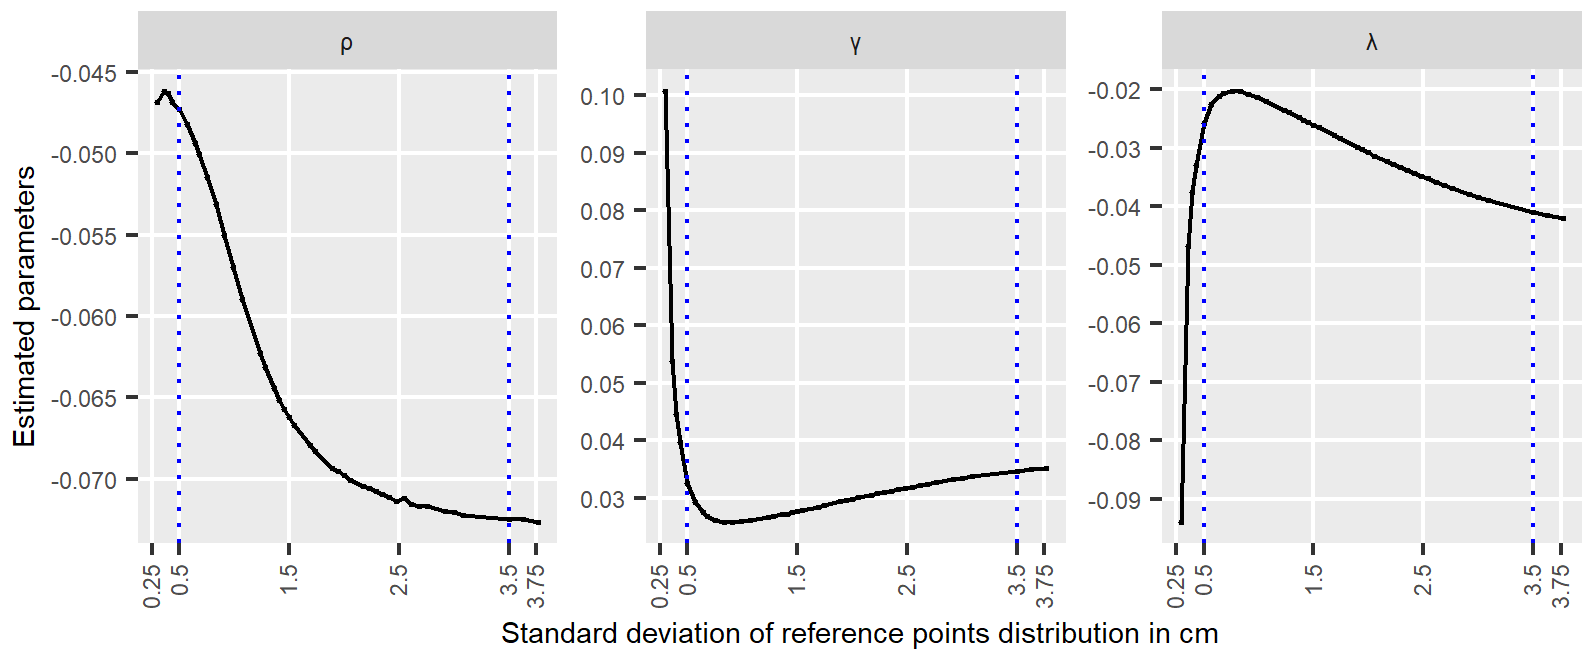
\includegraphics[width=1.10\textwidth]{tab_fig_online_appendix/fig_a2_estimates_final.png}}
\caption{Preference parameter estimates from estimating the model under different assumptions about the standard deviation of reference points distribution $\sigma_{R_{y,v}}$}
\label{fig:estimatesmulti}
\end{figure}

In Table \ref{tab:paramesti}, we present parameter estimates under four assumptions for $\sigma_{R_{y,v}}$ from 0.5 cm to 3.5 cm. In this section, for additional information, we provide key estimates from estimating the model at $\sigma_{R_{y,v}}$ values from 0.25 cm to 3.75 cm at 0.05 cm intervals. In Figure \ref{fig:estimatesmulti}, we visualize the point-estimates results for the core preference parameters of $\rho$, $\gamma$ and $\lambda$ in three sub-figures. We mark with dashed blue lines values of $\sigma_{R_{y,v}}$ along the x-axis where $\sigma_{R_{y,v}}=0.5$ and $\sigma_{R_{y,v}}=3.5$.

For $\rho$, the quadratic coefficient on non-nutritional consumptions, the estimated coefficient becomes more negative as $\sigma_{R_{y,v}}$ increases. This finding implies lower marginal gains from additional non-nutritional consumption at higher $\sigma_{R_{y,v}}$.

\clearpage
\pagebreak
\clearpage

\end{document}